%macbook 
\setcounter{paragraph}{0}
\PhanI
\begin{ex}%[3P2Y1-1][Loai1]
Một sóng dọc truyền trong một môi trường thì phương dao động của các phần tử môi trường
\choice
{là phương ngang}
{là phương thẳng đứng}
{\True trùng với phương truyền sóng}
{vuông góc với phương truyền sóng}
\loigiai{Một sóng dọc truyền trong một môi trường thì phương dao động của các phần tử môi trường trùng với phương truyền sóng}
\end{ex} \haidong{20}
\begin{ex}%[3P2Y1-1][Loai1]
Trong sự truyền sóng cơ, để phân loại sóng ngang và sóng dọc người ta căn cứ vào yếu tố nào sau đây?
\choice
{\True Phương dao động của phần tử vật chất và phương truyền sóng}
{Môi trường truyền sóng}
{Vận tốc truyền sóng}
{Phương dao động của phần tử vật chất}
\loigiai{Trong sự truyền sóng cơ, để phân loại sóng ngang và sóng dọc người ta căn cứ vào phương dao động của phần tử vật chất và phương truyền sóng}
\end{ex} \haidong{20}
\begin{ex}%[3P2Y1-1][Loai1]
Khi sóng ngang truyền qua một môi trường vật chất đàn hồi, các phần tử vật chất của môi trường sẽ
\choice
{\True dao động theo phương vuông góc phương truyền sóng với tần số bằng tần số dao động của nguồn sóng}
{dao động theo phương truyền sóng với vận tốc bằng vận tốc dao động của nguồn sóng}
{chuyển động theo phương vuông góc phương truyền sóng với vận tốc bằng vận tốc sóng}
{chuyển động theo phương truyền sóng với vận tốc bằng vận tốc sóng}
\loigiai{\begin{itemize}
\item A Đúng theo định nghĩa của sóng ngang.
\item Phần tử sóng không dao động hay chuyển động theo phương truyền sóng mà chỉ dao động xung quanh vị trí cân bằng trên phương vuông góc với phương truyền sóng và với vận tốc được xác định bằng $v=u'(t)$ nên B, C, D sai.
\end{itemize}}
\end{ex} \haidong{20}

\begin{ex}%CTST
\immini[thm]{
Hình bên mô tả hai loại sóng địa chấn truyền trong môi trường khi xảy ra động đất: sóng P (sóng sơ cấp) và sóng S (sóng thứ cấp). Phát biểu nào sau đây là đúng?
\choice
{P là sóng ngang, S là sóng dọc}
{P và S đều là sóng ngang}
{P và S đều là sóng dọc}
{\True P là sóng dọc, S là sóng ngang}
}{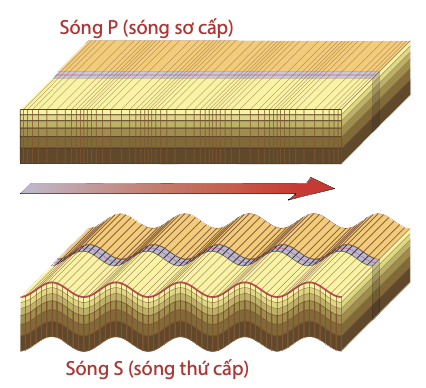
\includegraphics[width=4cm]{Hinh/CT5P2}}
\loigiai{
\begin{itemize}
\item Sóng P là sóng dọc vì các thớ địa chất dao động dọc theo phương truyền sóng.
\item Sóng S là sóng ngang vì các thớ địa chất dao động vuông góc với phương truyền sóng.
\end{itemize}
}
\end{ex} \haidong{20}


\begin{ex} %[3P2Y1-1][Loai1]
Đối với sóng cơ học thì sóng ngang truyền được
\choice
{trong chất rắn, chất lỏng và chất khí}
{trong chất rắn, trên bề mặt chất lỏng, trong chân không}
{\True trong chất rắn và trên bề mặt chất lỏng}
{trong các môi trường rắn và khí}
\loigiai{Sóng ngang truyền được trong chất rắn và trên bề mặt chất lỏng}
\end{ex} \haidong{20}


\begin{ex}%[3P2Y1-1][Loai1]
\nguon{QG - 2017} Trong sóng cơ, sóng dọc truyền được trong các môi trường
\choice
{rắn, khí và chân không}
{\True rắn, lỏng và khí}
{rắn, lỏng và chân không}
{lỏng, khí và chân không}
\loigiai{Sóng dọc cũng thuộc loại sóng cơ, chỉ truyền được trong môi trường rắn, lỏng, khí}
\end{ex} \haidong{20}
\begin{ex}%[3P2Y1-1][Loai1]
Phát biểu nào sau đây là đúng về sự truyền sóng cơ?
\choice
{Sóng cơ chỉ truyền được trong môi trường không khí}
{\True Sóng cơ truyền được trong môi trường rắn, lỏng, khí}
{Sóng cơ truyền được trong môi trường chân không}
{Sóng cơ chỉ truyền được trên vật rắn và mặt thoáng chất lỏng}
\loigiai{
Sóng cơ lan truyền được trong môi trường rắn, lỏng và khí.
}
\end{ex} \haidong{20}

\begin{ex}%[3P2Y1-1][Loai1]
\nguon{QG - 2017} Trong sóng cơ, tốc độ truyền sóng là
\choice
{tốc độ cực tiểu của các phần tử môi trường}
{tốc độ cực đại của các phần tử môi trường}
{\True tốc độ lan truyền dao động trong môi trường truyền sóng}
{tốc độ chuyển động của các phần tử môi trường truyền sóng}
\loigiai{Tốc độ truyền sóng là tốc độ lan truyền dao động cơ trong một môi trường}
\end{ex} \haidong{20}

\begin{ex}%[3P2Y1-1][Loai1]
Tốc độ truyền sóng phụ thuộc vào
\choice
{\True bản chất của môi trường}
{kích thước của môi trường}
{biên độ sóng}
{cường độ sóng}
\loigiai{
\begin{itemize}
\item 
Tốc độ truyền sóng phụ thuộc vào tính chất của môi trường: tính đàn hồi, mật độ vật chất và nhiệt độ của môi trường. 
\item Ví dụ như là môi trường có tính đàn hồi tốt thì sẽ truyền sóng tốt hơn.
\end{itemize}}
\end{ex} \haidong{20}
\begin{ex}
\immini[thm]{
Trong thí nghiệm ở hình, nếu ta thay đổi tần số dao động của nguồn sóng thì đại lượng nào sau đây không đổi?
\choice
{Chu kì sóng}
{Bước sóng}
{Tần số sóng}
{\True Tốc độ truyền sóng}
}{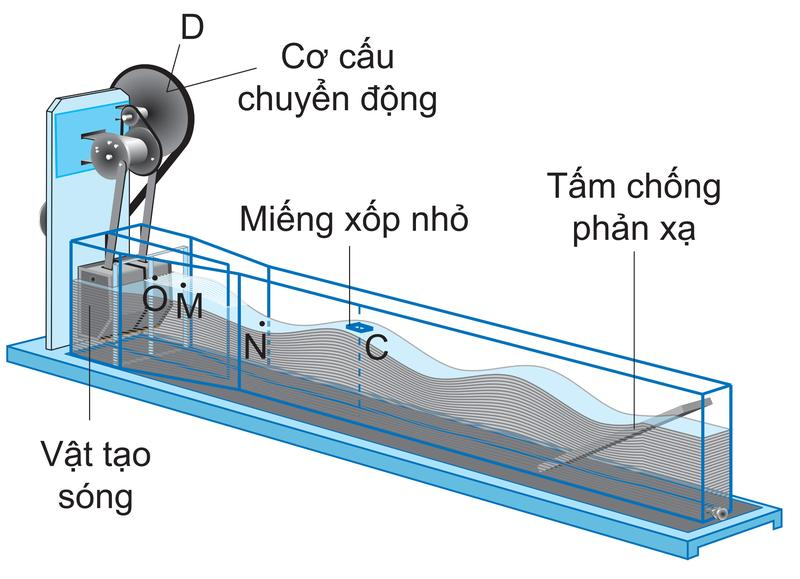
\includegraphics[width=4cm]{Hinh/KN81}}
\loigiai{
\begin{itemize}
\item Tốc độ truyền sóng chỉ phụ thuộc vào bản chất môi trường. 
\end{itemize}
}
\end{ex} \haidong{20}




\begin{ex}%[3P2Y1-1][Loai1]
\nguon{QG - 2019}
Một sóng cơ hình sin truyền dọc theo trục Ox. Quãng đường mà sóng truyền được trong một chu kì bằng
\choice
{nửa bước sóng}
{ba lần bước sóng}
{\True một bước sóng}
{hai lần bước sóng}
\loigiai{
Bước sóng là quãng đường sóng truyền được trong một chu kì.
}
\end{ex} \haidong{20}
\begin{ex}%[3P2Y2-1][Loai1]
Bước sóng là khoảng cách giữa hai điểm
\choice
{trên cùng một phương truyền sóng mà dao động tại hai điểm đó ngược pha}
{\True gần nhau nhất trên cùng một phương truyền sóng mà dao động tại hai điểm đó cùng pha}
{gần nhau nhất mà dao động tại hai điểm đó cùng pha}
{trên cùng một phương truyền sóng mà dao động tại hai điểm đó cùng pha}
\loigiai{Bước sóng là khoảng cách giữa hai điểm gần nhau nhất trên cùng một phương truyền sóng mà dao động tại hai điểm đó cùng pha}
\end{ex} \haidong{20}


\begin{ex}%[3P2B1-1][Loai1]
\nguon{QG - 2017} Khi một sóng cơ truyền từ không khí vào nước thì đại lượng nào sau đây không đổi?
\choice
{\True Tần số của sóng}
{Tốc độ truyền sóng}
{Bước sóng}
{Biên độ của sóng}
\loigiai{Khi sóng truyền từ môi trường này sang môi trường kia thì tần số của sóng luôn không đổi}
\end{ex} \haidong{20}




\begin{ex}%CTST
\immini[thm]{
Một cơn sóng truyền qua vị trí của phao câu cá đang nổi trên mặt nước như hình. Phao có trôi đi theo chiều truyền của sóng không?
\choice
{Phao trôi theo chiều truyền sóng}
{\True Phao không trôi theo chiều truyền sóng}
{Phao trôi ngược chiều truyền sóng}
{Phao trôi chéo so với phương truyền sóng}}{
\includegraphics[width=4cm]{Hinh/CT5P1}}
\loigiai{
\begin{itemize}
\item Phao chỉ dao động nhấp nhô tại chỗ chứ không trôi đi theo chiều truyền của sóng vì khi sóng truyền đi không mang theo các phần tử vật chất môi trường.
\end{itemize}
}
\end{ex} \haidong{20}
























 
 
 
 
 
 
 
 
 
 
 
 
 
 
 
 
 %macbook 
 
 \loai{Phân loại âm}
 \begin{ex}%[3P2YB-1][Loai1]
 	\nguon{MH - 2017} Tai con người có thể nghe được những âm có tần số nằm trong khoảng
 	\choice
 	{từ 16 kHz đến 20.000 Hz}
 	{từ 16 Hz đến 20.000 kHz}
 	{từ 16 kHz đến 20.000 kHz}
 	{\True từ 16 Hz đến 20.000 Hz}
 	\loigiai{
 		Tai người có thể nghe âm thanh có tần số 16 Hz đến 20000 Hz.
 	}
 \end{ex} \haidong{20}
 
 \begin{ex}%[3P2BB-1][Loai1]
 	Một lá thép mỏng, một đầu cố định, đầu còn lại được kích thích để dao động với chu kì không đổi và bằng 0,08 s. Âm do lá thép phát ra là
 	\choice
 	{âm mà tai người nghe được}
 	{nhạc âm}
 	{\True hạ âm}
 	{siêu âm}
 	\loigiai{
 		Tần số $f = \dfrac{1}{T} = 12\ Hz < 16 Hz \Rightarrow$ âm phát ra là hạ âm.
 	}
 \end{ex} \haidong{20}
 
 \loai{Sự truyền âm}
 \begin{ex}%[3P2BB-1][Loai1]
 	Một âm có tần số xác định truyền lần lượt trong nhôm, nước, không khí với tốc độ tương ứng là $v_1,\ v_2,\ v_3$. Nhận định nào sau đây là đúng?
 	\choice
 	{$v_2 > v_1 > v_3$}
 	{$v_3 > v_2 > v_1$}
 	{$v_1 > v_3 > v_2$}
 	{\True $v_1 > v_2 > v_3$}
 	\loigiai{
 		Tốc độ truyền âm giảm dần từ chất rắn đến lỏng đến khí.
 	}
 \end{ex} \haidong{20}

 
 
 
 
 
 \loai{Sóng âm truyền trong các môi trường}
 

 
 	\begin{ex}%[3P2BB-1][Loai1]
 		Sóng âm \textbf{không} có tính chất nào sau đây?
 		\choice
 		{Mang năng lượng tỉ lệ với bình phương biên độ sóng}
 		{Truyền được trong chất rắn, lỏng, khí}
 		{\True Là sóng ngang khi truyền trong chất khí}
 		{Có khả năng phản xạ, khúc xạ, giao thoa}
 		\loigiai{
 		}
 	\end{ex} \haidong{20}










\PhanII
\setcounter{ex}{0}
 	%Chuyển thành câu đúng sai
 	\begin{ex}
 		\immini[thm]{Khi thực hiện thí nghiệm truyền sóng âm đến dao động kí như hình vẽ, người ta sử dụng âm thoa và micro để thu và hiển thị tín hiệu âm. Xét tính đúng sai các phát biểu sau liên quan đến nguyên lý và điều kiện thực hiện thí nghiệm.}{
 			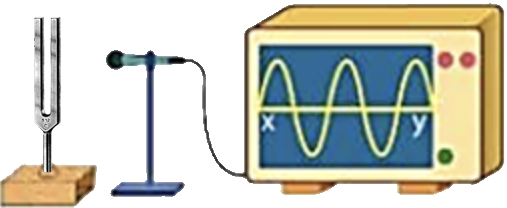
\includegraphics[width=5cm]{Hinh/KN104}
 		}
 		\choiceTF[t]
 		{\True Sóng âm từ âm thoa được truyền tới dao động kí thông qua micro thu}
 		{\True Dao động của âm thoa được chuyển thành dao động điện nhờ micro, đưa vào dao động kí hiển thị dạng sóng có cùng tần số}
 		{Tần số hiển thị trên dao động kí luôn cao hơn tần số dao động của âm thoa}
 		{\True Để giảm ảnh hưởng tiếng ồn, nên đặt thí nghiệm trong môi trường yên tĩnh và điều chỉnh micro thu chọn lọc âm}
 		\loigiai{
 			\begin{itemchoice}
 				\itemch Micro có vai trò chuyển dao động cơ (âm thanh) thành dao động điện, truyền tới dao động kí.
 				\itemch Tín hiệu điện có tần số trùng với âm thoa, nên đồ thị hiển thị phản ánh đúng dao động âm.
 				\itemch Nếu có nhiễu thì có thể làm sai lệch tín hiệu, nhưng khi hoạt động đúng thì tần số trên dao động kí bằng tần số âm thoa.
 				\itemch Giảm tiếng ồn và lọc tần số giúp thu chính xác tín hiệu cần đo từ âm thoa.
 			\end{itemchoice}
 		}
 	\end{ex}
 \begin{ex}
 	\immini[thm]{Khi đi biển, thủy thủ có thể dùng hệ thống sonar phát sóng siêu âm để định vị và tránh vật cản dưới nước. Trong tự nhiên, nhiều loài động vật như cá heo, cá voi cũng dùng sóng siêu âm để định vị và liên lạc. Xét các phát biểu sau về đặc điểm của kỹ thuật sonar và ảnh hưởng của nó đến sinh vật biển.}{
 		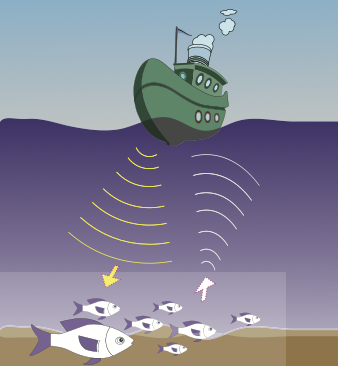
\includegraphics[width=5cm]{Hinh/CT6P1}
 	}
 	\choiceTF[t]
 	{\True Sonar hoạt động dựa trên sự phản xạ của sóng âm khi gặp vật cản dưới nước}
 	{\True Sóng siêu âm được dùng trong sonar vì trong môi trường nước thì sóng siêu âm ít bị suy giảm hơn sóng điện từ}
 	{Kỹ thuật sonar không ảnh hưởng đến cá voi và cá heo vì chúng không cảm nhận được sóng siêu âm}
 	{\True Cá voi và cá heo có thể bị rối loạn do sóng sonar của con người gây nhiễu hệ thống định vị sinh học của chúng}
 	\loigiai{
 		\begin{itemchoice}
 			\itemch Sonar phát sóng siêu âm, thu tín hiệu phản xạ để xác định vật cản dưới nước.
 			\itemch Sóng âm truyền trong nước với tốc độ lớn và ít suy giảm, còn sóng điện từ bị hấp thụ mạnh.
 			\itemch Sonar phát sóng mạnh có thể gây nhiễu biosonar của cá voi, cá heo, gây rối loạn định vị.
 			\itemch Nhiều nghiên cứu cho thấy sonar làm cá voi, cá heo mất phương hướng, thậm chí mắc cạn.
 		\end{itemchoice}
 	}
 \end{ex}
 	\begin{ex}
 	Tai người có thể tiếp nhận sóng âm trong một khoảng tần số nhất định gọi là vùng nghe. Âm thanh truyền đến tai làm rung màng nhĩ, được xử lí và cảm nhận thành âm cao hoặc thấp, to hoặc nhỏ.
 	\choiceTF[t]
 	{\True Sóng âm truyền đến tai người làm màng nhĩ dao động, do đó ta nghe được âm thanh}
 	{Biên độ sóng âm càng nhỏ thì âm nghe được càng lớn}
 	{\True Tần số sóng âm càng lớn thì âm nghe được càng cao}
 	{Dải tần số mà tai người có thể nghe được là từ $16 ~Hz$ đến $20000 ~Hz$. Biết tốc độ truyền âm trong không khí là $330 ~m/s$. Khi đó bước sóng bé nhất mà tai người nghe được là $19 ~m$}
 	\loigiai{
 		\begin{itemchoice}
 			\itemch
 			\itemch
 			\itemch
 			\itemch
 		\end{itemchoice}
 	}
 \end{ex} \haidong{20}
 	\begin{ex}
 		Trong đời sống và kĩ thuật, sóng là một cách truyền tải năng lượng rất phổ biến – từ sóng biển, sóng âm đến sóng điện từ. Xét các phát biểu sau về đặc điểm truyền năng lượng của sóng.
 		\choiceTF[t]
 		{\True Nguồn sóng là nguồn năng lượng}
 		{\True Sóng mang năng lượng của nguồn tới mọi nơi trên phương truyền sóng}
 		{\True Khi sóng truyền trên mặt nước, các phần tử nước chỉ dao động tại chỗ quanh vị trí cân bằng của chúng}
 		{Mọi sóng mang năng lượng đi xa, mang các phần tử vật chất đi cùng}
 		\loigiai{
 			\begin{itemchoice}
 				\itemch
 				\itemch
 				\itemch
 				\itemch Phần tử vật chất không di chuyển theo phương truyền sóng
 			\end{itemchoice}
 		}
 	\end{ex} \haidong{20}





